\section{The optical limit}\label{sec:13.5}

A photon of \SI{1.24}{eV} absorbed in silicon brings a momentum of \SI{1.24}{eV}, five parts in $10^4$ of the reciprocal-lattice scale $2\pi/a = \SI{2.28}{keV}$, so its phonon supplies all of the \SI{1.94}{keV} between hole and electron, while dark matter near the onset mass supplies \SI{0.9}{keV} or more itself (\cref{sec:13.1}). Both processes have the same final states, and the independent-particle loss function $L^{\mathrm{PA}}_{\mathrm{IP}}(\vect{q},\omega)$ of \cref{eq:13.3-LPA} describes both, at different momentum transfers. Its limit $\vect{q}\to0$ is the phonon-assisted absorption $\varepsilon_2^{\mathrm{PA}}(\omega)$ of \cref{eq:6.5-eps2PA}. The measured absorption edge then serves twice. It tests a computed $L^{\mathrm{PA}}$ at one end of its range of $\vect{q}$, and it enters the rate of dark-photon absorption directly, once it has been transferred from the temperature of the measurement to that of a detector.

\subsection{The small-momentum limit}

The limit cannot be taken term by term in the amplitude $M^\pm_{cv\nu}(\vect{k},\vect{q},\vect{Q})$ of \cref{eq:13.2-M}. Its intraband terms carry density vertices that tend to one and cancel at $\vect{q} = 0$ (\cref{eq:13.2-q0}), so the leading term in $q$ is a difference of large terms, each with a different expansion of the bands and vertices. The continuity equation avoids the expansion. For the full Hamiltonian of electrons and nuclei, \cref{eq:4.3-continuity} gives $[H, n_e(\vect{q})] = \vect{q}\cdot\vect{j}_e(\vect{q})$, exactly, and between any two eigenstates of $H$
\begin{equation*}
  (E_f - E_i)\,\langle f|n_e(\vect{q})|i\rangle = \langle f|\vect{q}\cdot\vect{j}_e(\vect{q})|i\rangle .
\end{equation*}
The second-order amplitude \cref{eq:13.2-T} is a matrix element of this kind. To first order in $H_{\mathrm{ep}}$ the eigenstates of $H$ are $|\tilde i\rangle = |i\rangle + \sum_m|m\rangle\langle m|H_{\mathrm{ep}}|i\rangle/(E_i - E_m)$ and $\langle\tilde f| = \langle f| + \sum_m\langle f|H_{\mathrm{ep}}|m\rangle\langle m|/(E_f - E_m)$, with unchanged energies, because $H_{\mathrm{ep}}$ changes the number of phonons by one and has no diagonal elements. With $E_f = E_i + \omega$, the part of $\langle\tilde f|n_e(\vect{q})|\tilde i\rangle$ linear in $H_{\mathrm{ep}}$ is \cref{eq:13.2-T} term by term. The same construction applied to $\vect{q}\cdot\vect{j}_e(\vect{q})$ gives its second-order amplitude, and the identity holds order by order on the energy shell:
\begin{equation}
  \omega\,\langle f|n_e^{(2)}(\vect{q})|i\rangle = \langle f|\bigl(\vect{q}\cdot\vect{j}_e(\vect{q})\bigr)^{(2)}|i\rangle .
  \label{eq:13.5-ward}
\end{equation}
The intermediate states must be off the shell for the expansion to exist, and the off-shell window of \cref{sec:13.2} guarantees it.

The current needs no cancellation. At $\vect{q} = 0$ it is the total velocity, $\vect{j}_e(0) = \sum_j\vect{p}_j/m_e = \op{\vect{V}}$ of \cref{eq:6.5-HA}, which conserves $\vect{k}$, and its second-order amplitude into the final state of \cref{eq:13.2-final} is the one that \cref{sec:6.5} computed for light, with the photon vertex $(e\mathcal{E}/2\omega)\,\hat{\vect{e}}_\gamma\cdot\op{\vect{V}}$ replaced by $\vect{q}\cdot\op{\vect{V}}$. The same four paths combine into one sum over every band. Write $M^\pm_{cv\nu}(\vect{k},\vect{Q};\hat{\vect{e}}_\gamma)$ for the optical amplitude \cref{eq:6.5-M} with its polarization shown. Then, with $\vect{j}_e(\vect{q}) = \op{\vect{V}} + O(q)$,
\begin{keyresult}[Optical limit of the phonon-assisted amplitude]
\begin{equation}
  M^\pm_{cv\nu}(\vect{k},\vect{q},\vect{Q}) = \frac{q}{\omega}\,M^\pm_{cv\nu}(\vect{k},\vect{Q};\hat{\vect{q}}) + O(q^2) ,
  \label{eq:13.5-Mlim}
\end{equation}
on the energy shell inside the off-shell window, with the final electron at $\vect{k}+\vect{Q}$ in the limit.
\end{keyresult}
\noindent At $\vect{q} = 0$ the right side vanishes, which is \cref{eq:13.2-q0}: the identity contains the cancellation of the intraband terms and needs no expansion of them. It also gives the amplitude its first power of $q$, as \cref{eq:3.2-optical} does for the zero-phonon vertex, with the transition energy $\omega$ in the denominator. For a single pair, $\rho_{cv} \to \vect{q}\cdot\vect{v}_{cv}/\omega$ on the shell; for a pair with a phonon, the velocity vertex is replaced by the whole second-order optical amplitude.

\Cref{eq:4.3-continuity} holds because the potential energy depends on positions alone. A nonlocal pseudopotential breaks this, and $[H, n_e(\vect{q})]$ acquires the commutator of the nonlocal part. The velocity then contains the term $\ii[V_{\mathrm{NL}},\vect{r}]$ of \cref{eq:3.2-dHk}, which first-principles optical calculations include. The electron--phonon vertex of a nonlocal potential, the derivative of $V_{\mathrm{NL}}$ with respect to a displacement, contributes a commutator of the same kind. It is a contact term, in which one vertex creates the phonon and couples to the field at once, and \cref{eq:13.5-ward} holds only if it is kept on the side of the current.

Inserted into the loss function \cref{eq:13.3-LPA}, \cref{eq:13.5-Mlim} multiplies the optical $|M^\pm|^2$ by $q^2/\omega^2$, and the factor $q^2$ cancels the $1/q^2$ of the Coulomb line. The prefactor becomes $8\pi^2\alpha/(\Omega\omega^2) = g_{\mathrm{deg}}\pi e^2/(\omega^2\Omega)$ with $g_{\mathrm{deg}} = 2$ and $e^2 = 4\pi\alpha$. The weights $w_\pm = (1 - \ee^{-\beta\omega})(n_{\vect{Q}\nu} + \frac12 \pm \frac12)$ become $n_{\vect{Q}\nu} + \frac12 \pm \frac12$, since $\beta\omega > 40$ at room temperature for $\omega$ near the gap. The energy delta function loses $\vect{q}$ from the electron's crystal momentum. What remains is \cref{eq:6.5-eps2PA} with the polarization $\hat{\vect{e}}_\gamma = \hat{\vect{q}}$:
\begin{keyresult}[Optical limit of the phonon-assisted loss function]
\begin{equation}
  \lim_{\vect{q}\to0}L^{\mathrm{PA}}_{\mathrm{IP}}(\vect{q},\omega) = \varepsilon_2^{\mathrm{PA}}(\omega)\big|_{\hat{\vect{e}}_\gamma = \hat{\vect{q}}} ,
  \label{eq:13.5-limit}
\end{equation}
for $T \ll \Eg$ and $\omega$ inside the off-shell window at $\vect{q}\to0$, that is, below the direct gap. In a crystal with a center of inversion $L^{\mathrm{PA}}_{\mathrm{IP}}(\vect{q},\omega) = L^{\mathrm{PA}}_{\mathrm{IP}}(-\vect{q},\omega)$, and the corrections are of relative order $q^2$.
\end{keyresult}
\noindent The optical result and its edge are derived in \cref{sec:6.5,app:D.18}. Near threshold, \cref{eq:13.5-limit} reduces to the Hall--Bardeen--Blatt edge \cref{eq:6.5-edge}~\cite{hall1954infrared}, the $q\to0$ form of the fixed-$\vect{q}$ law \cref{eq:13.3-near}. As $\vect{q}\to0$ the phonon wavevector $\vect{Q}^* = \vect{k}_{\mathrm{c}} - \vect{q}$ tends to $\vect{k}_{\mathrm{c}}$, the onset $\Eg + \omega_\nu(\vect{Q}^*)$ tends to the optical threshold $\Eg + \omega_\nu$, and $|M_\nu|^2/q^2$ to the optical $|M_\nu|^2/\omega^2$. The full formula is the one that first-principles calculations of the absorption of silicon evaluate~\cite[Eq.~(1)]{noffsinger2012phonon}.

\subsection{Longitudinal and transverse absorption}

\Cref{eq:13.5-limit} selects the polarization along $\vect{q}$, the longitudinal one. A photon is transverse, and the measured absorption is $\varepsilon_2^{\mathrm{PA}}$ for $\hat{\vect{e}}_\gamma \perp \vect{q}$. Both are projections of one tensor. The amplitude is linear in the polarization, $M^\pm(\vect{k},\vect{Q};\hat{\vect{e}}) = \hat{e}^\alpha M^{\pm\alpha}$, and \cref{eq:6.5-eps2PA} is $\hat{e}^\alpha\hat{e}^\beta\varepsilon_2^{\mathrm{PA},\alpha\beta}(\omega)$, with the tensor built from $M^{\pm\alpha}M^{\pm\beta*}$ under the same double zone average. That average runs over every $\vect{k}$ and $\vect{Q}$ of the zone, every band and every branch, and the thermal state of the phonons is invariant under the point group. The tensor therefore commutes with every operation of the cubic group, and in silicon it is a multiple of the unit matrix (\cref{app:C.3}). The phonon-assisted part obeys \cref{eq:4.4-ET} by itself:
\begin{equation*}
  \varepsilon_2^{\mathrm{PA,T}}(\omega) = \varepsilon_2^{\mathrm{PA,L}}(\omega) = \varepsilon_2^{\mathrm{PA}}(\omega) \qquad (\vect{q}\to0) .
\end{equation*}
The equality holds for the summed tensor, not transition by transition: a single valley and branch contributes an anisotropic tensor, and the six valleys together restore the cubic symmetry.

The measured absorption between the indirect and the direct gap is therefore the longitudinal $\varepsilon_2^{\mathrm{PA}}$ at $\vect{q}\to0$ and at the temperature of the measurement. With the other electrons polarizing the medium, the longitudinal loss function is $\varepsilon_2^{\mathrm{PA}}/(\varepsilon_1^0)^2$ (\cref{eq:13.4-Lscr}). \Cref{eq:13.5-limit} holds for the screened amplitude $\tilde M^\pm$ as well, pair channel included, since the continuity argument uses only the energy shell; the measured $\varepsilon_2^{\mathrm{PA}}$ contains every screening effect of the amplitude at $\vect{q}\to0$, though not the external factor. At the edge of silicon $\varepsilon_1^0 = n_r^2 = 12.8$ at \SI{1.24}{eV}~\cite{franta2017temperature}, and $\varepsilon_2$ stays below $10^{-2}$ within \SI{0.2}{eV} of the gap, so this is the edge part of $\varepsilon_2/|\varepsilon|^2$, the loss function that sets the dark-photon rate \cref{eq:10.7-dp}. A dark photon of mass $m_\phi$ in the halo carries $|\vect{p}_\phi| \approx 10^{-3}m_\phi$, about \SI{1}{meV} at the edge, and sits at $|\vect{p}_\phi|/(2\pi/a) \approx 5\times10^{-7}$. Its longitudinal and transverse modes both absorb with the measured $\varepsilon_2^{\mathrm{PA}}$, and the corrections of order $q^2$ are negligible. Its rate at the edge, with the phonon-assisted absorption of bosonic dark matter in general, is the subject of \cref{sec:13.8}.

\subsection{The measured edge as a test}

\Cref{eq:13.5-limit} turns every measured absorption spectrum of silicon below \SI{3.4}{eV} into a test of a computed $L^{\mathrm{PA}}$ at one end of its domain. The test runs forward: the calculation is done at the temperature of the measurement, with the occupations $n_{\vect{Q}\nu}(T)$ and the gap $\Eg(T)$ of that temperature, and compared with the data. First-principles calculations of the silicon edge at \SIrange{249}{415}{K} agree with the measured spectra at every temperature, once the computed spectra are shifted rigidly by \SIrange{0.15}{0.23}{eV} to correct the computed gap~\cite{noffsinger2012phonon}. The simplest form of the limit is the edge of \cref{eq:6.5-edge} with free pairs, parabolic bands and constant matrix elements. With the branch weights $A_{\mathrm{TA}}:A_{\mathrm{TO}} = 5.5:4.0$ of a fit to the measured edge~\cite{rajkanan1979absorption,stanford2021photoelectric} and one overall scale fitted to the data between 1.18 and \SI{1.30}{eV}, it lies within \SI{15}{\percent} of the measured absorption at \SI{300}{K}~\cite{franta2017temperature} from 55 to \SI{490}{meV} above the gap (\cref{fig:13-transfer}). Closer to the gap the data exceed the edge formula, by a factor of 1.4 at \SI{36}{meV} and of 2 at \SI{17}{meV}; above about \SI{0.5}{eV} the matrix elements and bands vary across the zone, and above \SI{2.5}{eV} new thresholds open.

The constant matrix element is an approximation of the edge formula, not of \cref{eq:13.5-limit}: the full $\varepsilon_2^{\mathrm{PA}}$ keeps $M^\pm$ at every $\vect{k}$ and $\vect{Q}$, and only a calculation of it can follow the data above \SI{0.5}{eV}. Near the gap the excess is the electron--hole attraction, which the independent-particle $L^{\mathrm{PA}}$ leaves out. The bound pair lies $E_x^b = \SI{14.7}{meV}$ below the gap at the crystal momentum of the valley, every threshold has an excitonic companion that much lower (\cref{sec:6.5}), and a calculation that is to match the edge within a few tens of meV must include it (\cref{sec:13.8}).

\subsection{Temperature transfer of absorption data}

The measured edge is also an input. A dark photon absorbed between the indirect and the direct gap of a detector at \SI{10}{mK} sees the phonon-assisted $\varepsilon_2$ of cold silicon. Continuous spectra of the edge are measured at \SI{300}{K} or at \SI{77}{K}; the one measurement below \SI{1}{K} covers a few discrete photon energies from \SI{1.21}{eV} up~\cite{stanford2021photoelectric}. Projections for silicon detectors have used the \SI{77}{K} data near the gap~\cite{hochberg2017absorption}. \Cref{eq:6.5-eps2PA} contains the temperature in two places, the occupations and the gap, and between them they change the edge by large factors (\cref{sec:10.7-edge}).

Take one branch $\nu$ and write $\alpha_{\mathrm{abs},\nu}(\omega;T)$ for its part of the absorption. It consists of an emission component with weight $n_\nu + 1$ and an absorption component with weight $n_\nu$, both functions of the pair energy above the gap, $\omega - \Eg(T) \mp \omega_\nu$. Assume that the spectrum of the pairs, the matrix elements and the phonon energy do not change with temperature, and that the gap moves rigidly by $\Delta E_{\mathrm{g}}(T) = \Eg(T) - \Eg(0) < 0$. At $T \to 0$ only emission survives, and that spectrum is $\alpha^0_{\mathrm{abs},\nu}(\omega)$. At temperature $T$,
\begin{equation}
  \alpha_{\mathrm{abs},\nu}(\omega;T) = (n_\nu + 1)\,\alpha^0_{\mathrm{abs},\nu}\bigl(\omega - \Delta E_{\mathrm{g}}\bigr) + n_\nu\,\alpha^0_{\mathrm{abs},\nu}\bigl(\omega - \Delta E_{\mathrm{g}} + 2\omega_\nu\bigr) ,
  \label{eq:13.5-forward}
\end{equation}
which is \cref{eq:6.5-edge} with a general spectrum in place of the square. The emission term is the cold spectrum moved down by the gap shift; the absorption term is the same spectrum moved down by a further $2\omega_\nu$.

\Cref{eq:13.5-forward} can be solved for the cold spectrum. Evaluate it at $\omega + \Delta E_{\mathrm{g}}$ and divide by $n_\nu + 1$:
\begin{equation*}
  \alpha^0_{\mathrm{abs},\nu}(\omega) = \frac{\alpha_{\mathrm{abs},\nu}(\omega + \Delta E_{\mathrm{g}};T)}{n_\nu + 1} - \frac{n_\nu}{n_\nu + 1}\,\alpha^0_{\mathrm{abs},\nu}(\omega + 2\omega_\nu) .
\end{equation*}
The unknown reappears on the right at an energy higher by $2\omega_\nu$, with the factor $n_\nu/(n_\nu + 1) = \ee^{-\omega_\nu/T}$ of detailed balance (\cref{eq:6.5-ratio}). Substituting the equation into itself and using $1/(n_\nu + 1) = 1 - \ee^{-\omega_\nu/T}$,
\begin{keyresult}[Inverse temperature transfer]
\begin{equation}
  \alpha^0_{\mathrm{abs},\nu}(\omega) = \bigl(1 - \ee^{-\omega_\nu/T}\bigr)\sum_{k=0}^{\infty}\bigl(-\ee^{-\omega_\nu/T}\bigr)^k\,\alpha_{\mathrm{abs},\nu}\bigl(\omega + \Delta E_{\mathrm{g}}(T) + 2k\,\omega_\nu;\,T\bigr) ,
  \label{eq:13.5-inverse}
\end{equation}
exact for the spectrum of one branch measured at the temperature $T$, under the assumptions of \cref{eq:13.5-forward}. The cold absorption is $\sum_\nu\alpha^0_{\mathrm{abs},\nu}$, and the dark-photon rate \cref{eq:10.7-dp} scales with it.
\end{keyresult}
\noindent The series converges geometrically at any temperature, with ratio $\ee^{-\omega_\nu/T}$: 0.064 for the transverse acoustic branch at \SI{77}{K}, $1.7\times10^{-4}$ for the transverse optical one, and 0.49 and 0.11 at \SI{300}{K}. It needs the data up to a few times $2\omega_\nu$ above $\omega$, and it is the unique solution that vanishes below the cold threshold. Each of the assumptions is a property of the spectrum, not of the inversion.

The inversion needs the spectrum of each branch separately, and a measured spectrum is their sum. One spectrum cannot fix two unknown functions. The triangular structure of \cref{eq:13.5-forward} does allow a solution that starts at the lowest threshold and works upward, but the term with the highest argument at each energy is the absorption replica of the transverse optical branch. Each step of that solution divides by its occupation, $n_{\mathrm{TO}} = 1.7\times10^{-4}$ at \SI{77}{K}, and multiplies every error in the data by $\ee^{\omega_{\mathrm{TO}}/T} = 6\times10^3$. At \SI{300}{K} the factor is 9.3. Without spectra resolved by branch, the transfer is therefore ill-posed: the data at one temperature leave the decomposition, and with it the cold spectrum, undetermined. The branch weights must come from elsewhere, from low-temperature spectra in which each threshold is resolved, as in the edge spectroscopy of \cref{sec:6.5}, or from a calculation of $\varepsilon_2^{\mathrm{PA}}$ branch by branch. The cold spectrum inherits their error. From \SI{77}{K} data the inheritance is mild, because only the transverse acoustic branch is occupied: with its weight changed by \SI{25}{\percent} either way, the transferred spectrum changes by less than \SI{1}{\percent} at 15 and \SI{50}{meV} above the cold threshold. From \SI{300}{K} data it changes by $-29$ and $+18$ percent at \SI{15}{meV}.

\begin{figure}[tbp]
  \centering
  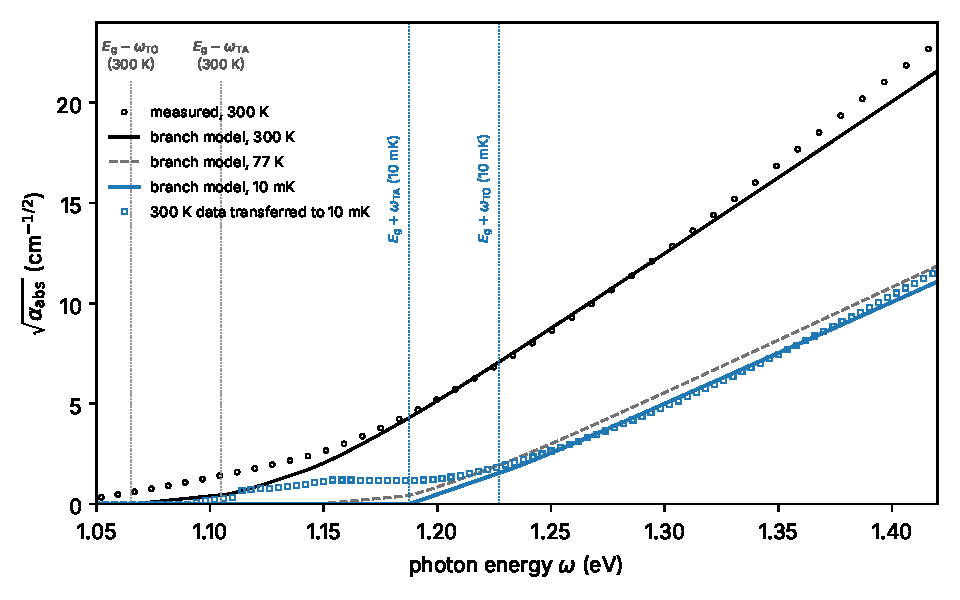
\includegraphics[width=0.92\linewidth]{figures/ch13/fig13_5.pdf}
  \caption{The absorption edge of silicon, as $\sqrt{\alpha_{\mathrm{abs}}}$ against the photon energy, at \SI{300}{K} and transferred to \SI{10}{mK}. Circles: measured at \SI{300}{K}~\cite{franta2017temperature}. Lines: a two-branch model of the edge. It has free pairs with the Hall--Bardeen--Blatt form of \cref{eq:6.5-edge}, $\omega_{\mathrm{TA}} = \SI{18.27}{meV}$ and $\omega_{\mathrm{TO}} = \SI{57.73}{meV}$, branch weights $5.5:4.0$~\cite{rajkanan1979absorption,stanford2021photoelectric}. The gap is the measured $\Eg(T)$ of \cref{sec:6.3}, 1.1692, 1.1652 and \SI{1.1230}{eV} at 0, 77 and \SI{300}{K}, with one scale fitted to the \SI{300}{K} data between 1.18 and \SI{1.30}{eV}. It is drawn at \SI{300}{K} (black), \SI{77}{K} (gray, dashed) and \SI{10}{mK} (blue). Squares: the \SI{300}{K} data transferred to \SI{10}{mK} with \cref{eq:13.5-inverse}, each energy split between the branches in the proportion of the model. Dotted: the thresholds $\Eg - \omega_\nu$ of phonon absorption at \SI{300}{K} and the emission thresholds $\Eg + \omega_\nu$ of cold silicon. Excitonic thresholds, \SI{14.7}{meV} below the free-pair ones, are not modeled.}
  \label{fig:13-transfer}
\end{figure}

\Cref{fig:13-transfer} shows the transfer for silicon. The warm edge starts \SI{57.7}{meV} below the \SI{300}{K} gap of \SI{1.123}{eV}, with the absorption replica of the transverse optical branch, and the cold one at $\Eg(0) + \omega_{\mathrm{TA}} = \SI{1.1875}{eV}$, \SI{0.12}{eV} higher; at \SI{1.236}{eV} the measured \SI{300}{K} absorption, \SI{58}{cm^{-1}}, is 16 times the cold one. Transferred, the data follow the cold model above \SI{1.25}{eV} to within \SI{10}{\percent}, the accuracy with which the model follows the warm data. Below the cold threshold they keep about \SI{1.4}{cm^{-1}}, where cold silicon absorbs nothing outside the excitonic thresholds. That residue is the part of the \SI{300}{K} data that is not of the form \cref{eq:13.5-forward} assumes, the excitonic companions and the thermal broadening of the warm edge, and the inversion carries it to the cold side unchanged in size. Near the cold threshold the transfer of room-temperature data is no better than this residue.

The assumption of a temperature-independent spectrum fails at a level that measurements show. Stanford and co-workers measured the absorption of silicon at 0.5, 5, 77 and \SI{295}{K} and fitted the two-branch form to it with an effective gap of \SI{1.134}{eV}. The fit needs a branch strength that falls with temperature as $\ee^{-c_1T}$ with $c_1 = \SI{1.7e-3}{K^{-1}}$~\cite[Eqs.~(6) and (7)]{stanford2021photoelectric}: a factor 0.61 at \SI{295}{K} and 0.88 at \SI{77}{K}, relative to the lowest temperature, within their own law for the gap, which differs slightly from the one used here. The occupations and a rigid gap do not carry all of the temperature dependence. The bands are renormalized by the lattice vibrations, not only shifted (\cref{sec:6.3}), and the vertices change with them (\cref{sec:13.7}). Transferred with \cref{eq:13.5-inverse}, \SI{295}{K} data therefore underestimate the cold spectrum by about \SI{40}{\percent} on this evidence, and \SI{77}{K} data by about \SI{12}{\percent}, with the opposite sign to the errors of the untransferred data.

\begin{keyresult}[Untransferred \SI{77}{K} data]
Used without transfer, the \SI{77}{K} absorption of silicon overestimates the millikelvin dark-photon rate by the factors
\begin{equation*}
  2.3\text{--}2.6,\quad 1.7\text{--}1.9,\quad 1.3\text{--}1.5,\quad 1.1\text{--}1.3 \qquad \text{at} \qquad x = 15,\ 25,\ 50,\ \SI{100}{meV} ,
\end{equation*}
where $x$ is the energy above the cold threshold $\Eg(0) + \omega_{\mathrm{TA}}$, and by more than a factor of two for $x$ below 18 to \SI{23}{meV}. The upper values hold for the transverse acoustic branch alone and for the two-branch edge to two digits; the lower ones include the measured fall of the branch strength between the lowest temperature and \SI{77}{K}. Untransferred \SI{300}{K} data overestimate the two-branch edge by 38, 16 and 7 at $x = 25$, 50 and \SI{100}{meV}.
\end{keyresult}
\noindent The two causes add. The \SI{77}{K} gap lies \SI{3.97}{meV} below the cold one, so that at the same photon energy the warm emission edge has run $x + \SI{3.97}{meV}$. And the transverse acoustic phonon is still occupied, $n_{\mathrm{TA}} = 0.068$, which adds stimulated emission and an absorption replica that starts $2\omega_{\mathrm{TA}}$ lower. The gap shift dominates close to the threshold, where $(1 + |\Delta E_{\mathrm{g}}|/x)^2$ is large, and the occupation farther away. The factors belong to the free-pair edge, whose power two is the steepest at the threshold. An excitonic edge rises more slowly and its gap-shift factor is smaller. The lower values of the box follow from the branch strength at \SI{77}{K}, lower than the cold one by the factor 0.88 above, which moves the factor of two from $x = 23$ to \SI{18}{meV}. These are the corrections that the silicon dark-photon rate of \cref{sec:10.7-edge} needs near its edge, and they apply to every absorption rate of \cref{chap:10} that uses measured $\sigma_1$ below the direct gap.

\begin{workedexample}{The transverse acoustic correction at 50 meV}\label{we:13-TA-transfer}
Take the transverse acoustic component of the silicon edge at $x = \SI{50}{meV}$ above the cold threshold, $\omega = \Eg(0) + \omega_{\mathrm{TA}} + x = \SI{1.2375}{eV}$, with $\Eg(0) = \SI{1.1692}{eV}$ and $\omega_{\mathrm{TA}} = \SI{18.27}{meV}$, and its \SI{77}{K} spectrum, with $\Eg(\SI{77}{K}) = \SI{1.1652}{eV}$ ($\Delta E_{\mathrm{g}} = \SI{-3.97}{meV}$) and $n_{\mathrm{TA}} = 0.0681$. In the edge form the cold component is $A\,x^2$.

\emph{Forward.} At \SI{77}{K} the emission component has run $\omega - \Eg(\SI{77}{K}) - \omega_{\mathrm{TA}} = \SI{53.97}{meV}$, and the absorption component $\omega - \Eg(\SI{77}{K}) + \omega_{\mathrm{TA}} = \SI{90.50}{meV}$. Relative to the cold value $A\,(\SI{50}{meV})^2$,
\begin{equation*}
  \underbrace{(n_{\mathrm{TA}} + 1)}_{1.0681}\underbrace{\Bigl(\frac{53.97}{50}\Bigr)^2}_{1.1651} + \underbrace{n_{\mathrm{TA}}}_{0.0681}\underbrace{\Bigl(\frac{90.50}{50}\Bigr)^2}_{3.276} = 1.2443 + 0.2230 = 1.467 .
\end{equation*}
The gap shift alone gives \SI{17}{\percent}, stimulated emission multiplies it by 1.068, and the absorption replica adds 0.22: the \SI{77}{K} spectrum is 1.47 times the cold one at this energy.

\emph{Inverse.} \Cref{eq:13.5-inverse} with $\ee^{-\omega_{\mathrm{TA}}/T} = 0.0637$ reads the \SI{77}{K} spectrum at $\omega + \Delta E_{\mathrm{g}} + 2k\omega_{\mathrm{TA}} = 1.2335$, 1.2700, 1.3066, 1.3431, \SI{1.3796}{eV}. In units of the cold value, the terms are
\begin{equation*}
  +1.19087,\quad -0.21547,\quad +0.02724,\quad -0.00289,\quad +0.00028 ,
\end{equation*}
and the partial sums 1.19087, 0.97540, 1.00264, 0.99975, 1.00002. The first term alone, the gap-shifted spectrum divided by $n_{\mathrm{TA}} + 1$, is \SI{19}{\percent} high, because it still contains the absorption replica; the second removes it, and each further term corrects the previous one by a factor $\ee^{-\omega_{\mathrm{TA}}/T}$ and a ratio of squares. Five terms recover the cold value to $2\times10^{-5}$.
\end{workedexample}

\subsection{Finite-momentum corrections}

A dark-matter particle that scatters never reaches the optical limit. To deposit $\omega$ it must transfer at least $q = \omega/v_{\mathrm{max}}$, \SI{0.45}{keV} at the silicon edge with $v_{\mathrm{max}} = 2.65\times10^{-3}$, and in the phonon-assisted window it transfers \SIrange{0.9}{1.3}{keV} (\cref{sec:13.1,sec:13.3}), $0.4$ to $0.6$ of $2\pi/a$. At such $\vect{q}$ the corrections of \cref{eq:13.5-limit} are not small, for three reasons outside the reach of optical data. The intermediate states of path A sit at $\vect{k}+\vect{q}$, and their energy moves by an amount of order $q^2/2m_e$, \SI{0.98}{eV} at \SI{1}{keV}, against a distance from the energy shell of $E_{\mathrm{dir}} - \omega \approx \SI{2.2}{eV}$ at the edge. The density vertices $\rho_{pv}(\vect{k},\vect{q})$ depart from their linear form \cref{eq:3.2-optical} on the scale of $2\pi/a = \SI{2.28}{keV}$, and beyond that a reciprocal-lattice vector inside the vertex reaches valleys that no photon reaches, as the class $(2\pi/a)(2,0,0)$ of \cref{sec:13.3} does, with its own selection rules. And the phonon itself is a different one: at $\vect{q} \to 0$ it carries $\vect{k}_{\mathrm{c}}$, where the transverse acoustic branch is at \SI{18.27}{meV}, while at $|\vect{q}| = \SI{1.0}{keV}$ along the valley axis it carries $\vect{k}_{\mathrm{c}} - \vect{q}$, at $0.41\,\mathrm{X}$, and the computed branch is at \SI{13.98}{meV} (\cref{we:13-onset-exp}). The optical edge measures the electron--phonon vertices only at $\vect{Q} \approx \vect{k}_{\mathrm{c}}$.

The optical limit therefore tests the parts of a calculation that do not depend on $\vect{q}$: the bands at the extrema, the gap, the electron--phonon vertices near $\vect{k}_{\mathrm{c}}$, the unrestricted sum over intermediate bands with its intraband terms, and the normalization of \cref{eq:13.3-LPA}. It does not test the finite-$\vect{q}$ density vertex, the Umklapp classes, the local fields or the vertices at $\vect{k}_{\mathrm{c}} - \vect{q}$, and these carry the dark-matter scattering rate. A computed $L^{\mathrm{PA}}(\vect{q},\omega)$ that reproduces the measured edge at the temperature of the measurement has passed a necessary check. The finite-$\vect{q}$ structure has to be controlled by sum rules and convergence tests.
